\documentclass[../main.tex]{subfiles}
\graphicspath{{\subfix{../media/}}}


\begin{document}
	
	\begin{figure}[h]
	    \centering
	    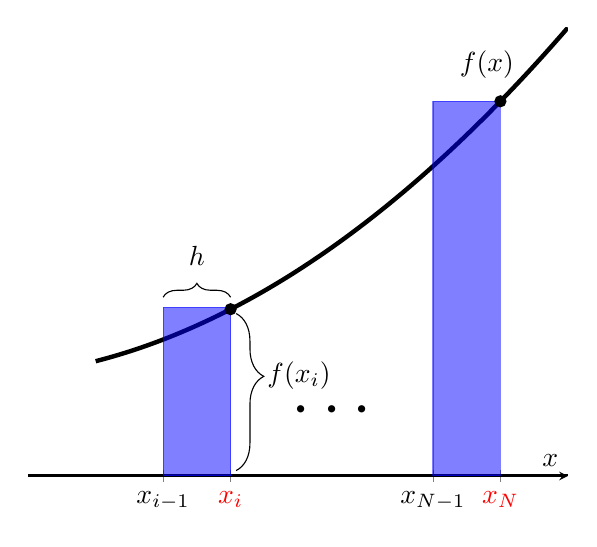
\begin{tikzpicture}
	        % Points stencil
	        \def\pointx{2}
	        \def\pointh{3.5}
	        
	        \begin{axis}[
	            xlabel = $x$,
	            ylabel = $f(x)$,
	            hide y axis,
	            xtick = {3, 4, 7, 8},
	            xticklabels = {$x_{i-1}$, \textcolor{red}{$x_i$}, $x_{N-1}$, \textcolor{red}{$x_N$}},
	            axis lines = middle,  
	            declare function={
	                func(\x) = 0.4*\x^2 + 9;
	            }
	        ]
	            
	            % Function
	            \addplot[ultra thick, domain=2:9, samples=100, label={center:$f(x)$}] {func(x)};
	            \addplot[ultra thick, domain=1:9, samples=2] {0};
	            \addplot[samples at={4, 8}, mark=*, only marks] {func(x)};

				% Reimann rectangles
                \filldraw[blue, opacity=0.5] (axis cs: 3,0) rectangle (axis cs: 4,15.6);
                \filldraw[blue, opacity=0.5] (axis cs: 7,0) rectangle (axis cs: 8,34.6);

				% decoration
				\draw [decorate, decoration={brace,amplitude=10pt,raise=2pt, aspect=0.4}] (axis cs:4,15) -- (axis cs:4,0.5) node [midway, anchor=west, yshift=6pt, outer sep=10pt]{$f(x_i)$};
				\draw [decorate, decoration={brace,amplitude=5pt,raise=2pt}] (axis cs:3,16) -- (axis cs:4,16) node [midway, anchor=south, outer sep=10pt]{$h$};          

	            % Nodes for x values
	            \node[name=nodeA] at (axis cs: 5.5, 6) {\Huge$\cdots$};
	            \node[name=nodeB] at (axis cs: 7.8, 38) {$f(x)$};

	        \end{axis}
	    \end{tikzpicture}
	    \caption{Rectangle Method Right Point Rule}
	\end{figure}
	
\end{document}